\chapter{Effective Mass and the Semiconductor Carrier Model}
\label{ch:effective-mass-carrier-model}

The Drude--Sommerfeld model describes carriers with a prescribed dispersion and
relaxation time.  A crystal supplies that dispersion through its Bloch bands.
Band gradients determine velocity, band curvature determines effective mass,
and equilibrium occupation determines the electron and hole populations.  The
resulting density moments form the semiconductor drift--diffusion model.

\section{Crystal bands and effective mass}

A carrier in a crystal responds to band curvature rather than to the vacuum
mass alone.  The semiclassical acceleration theorem is
\begin{equation}
  \hbar\dot{\bm k}=q_c\bm E.
  \label{eq:carrier-acceleration-theorem}
\end{equation}
Differentiating \cref{eq:sommerfeld-band-velocity} gives
\begin{equation}
  \dot{\bm v}=q_c\bm M^{*-1}\bm E,
  \qquad
  \left(\bm M^{*-1}\right)_{ij}
  =\frac1{\hbar^2}
   \frac{\partial^2E}{\partial k_i\partial k_j}.
  \label{eq:carrier-effective-mass-dynamics}
\end{equation}
This tensor is the effective mass already derived from band-edge curvature in
\cref{eq:conduction-inverse-effective-mass}.

For a parabolic band and scalar relaxation time, the tensor Drude relations are
\begin{equation}
  \boxed{
  \bm\mu=|q_c|\tau\bm M^{*-1},
  \qquad
  \bm D=\kb T\tau\bm M^{*-1},
  \qquad
  \bm\sigma=nq_c^2\tau\bm M^{*-1}.
  }
  \label{eq:carrier-effective-mass-transport}
\end{equation}
The Maxwell--Boltzmann velocity covariance becomes
\begin{equation}
  \left\langle\bm V\bm V^{\mathsf T}\right\rangle
  =\kb T\bm M^{*-1}.
  \label{eq:carrier-effective-mass-covariance}
\end{equation}
The density-of-states mass controls the equilibrium population.  The
conductivity mass controls acceleration, mobility, and current.  Anisotropic or
multivalley bands require the full inverse-mass tensors and the population of
each valley.

\begin{figure}[htbp]
  \centering
  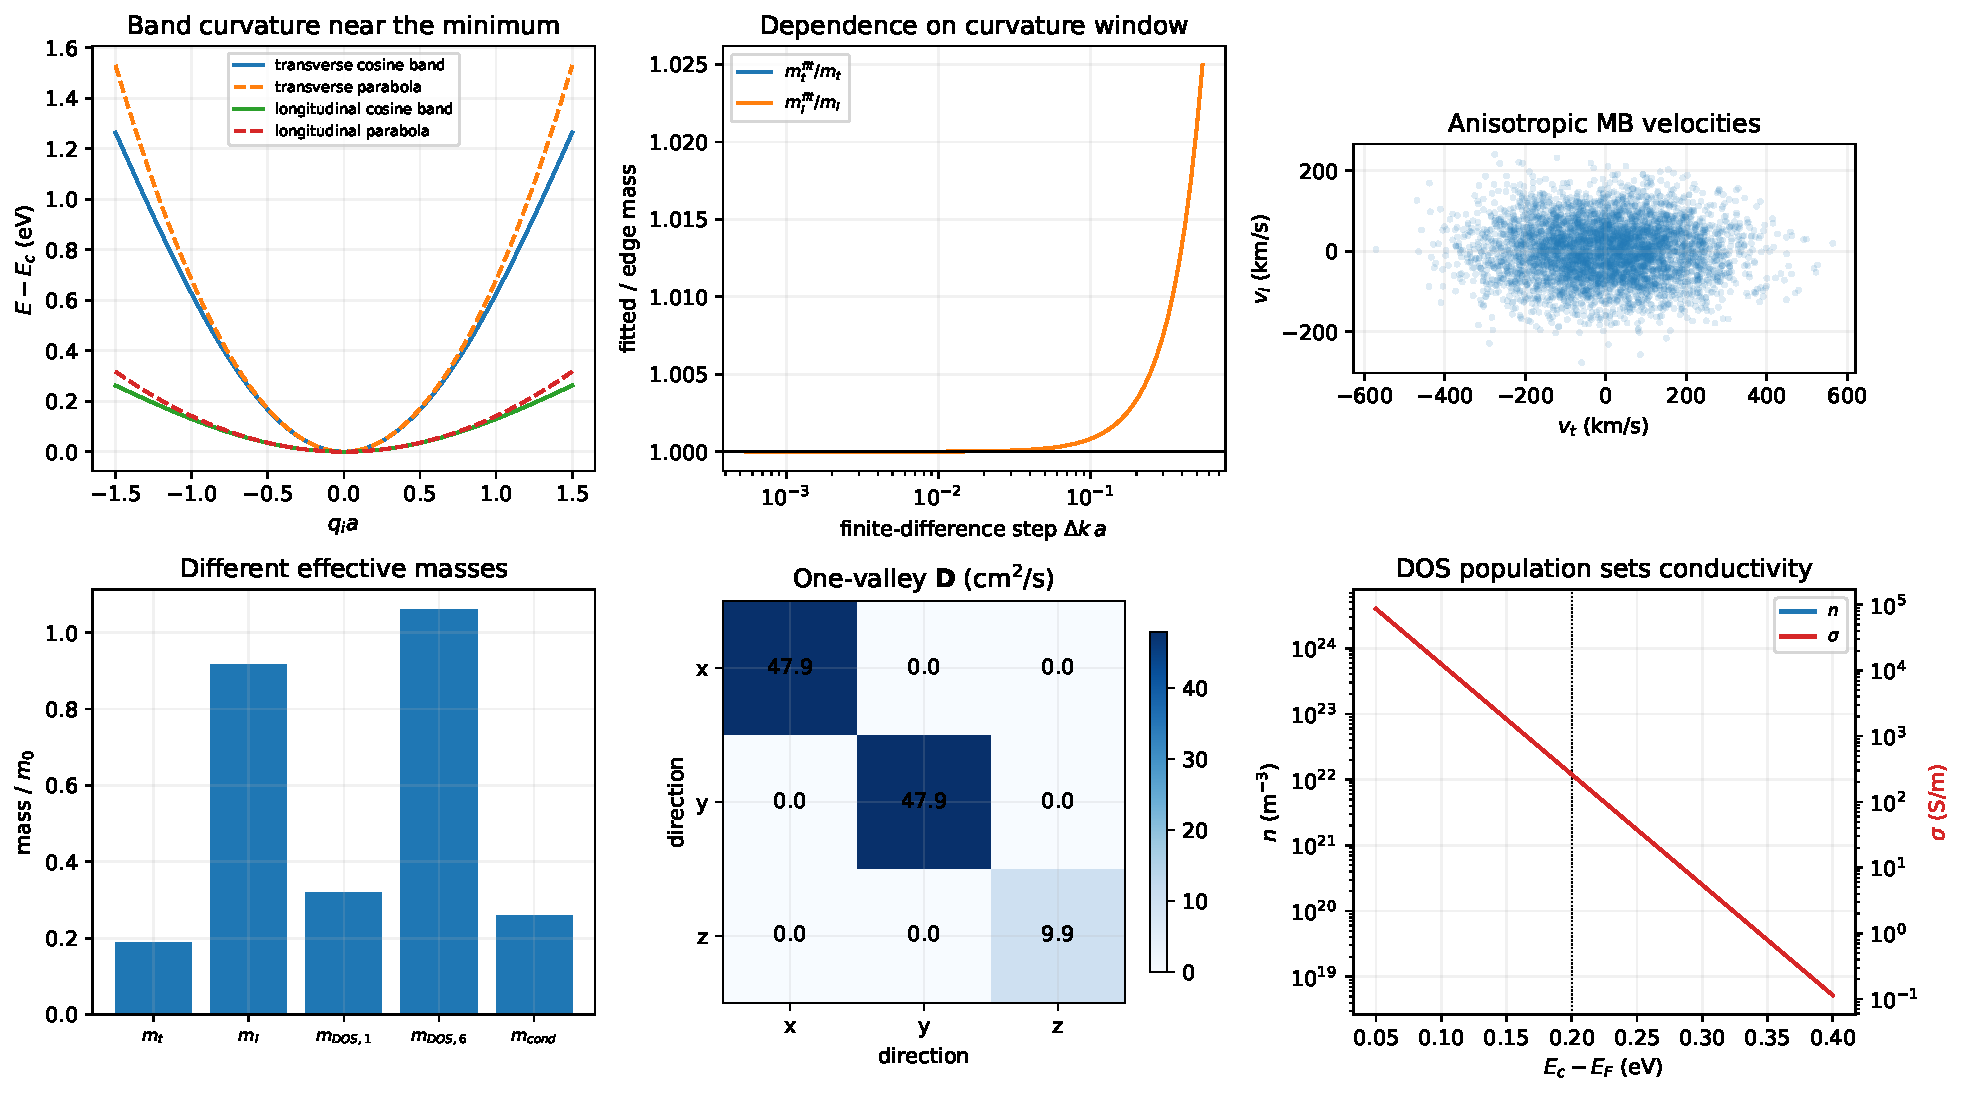
\includegraphics[width=\textwidth]
    {figures/08_brownian-motion-diffusion/lab-05-effective-mass-from-bands-to-transport.pdf}
  \caption{Band curvature determines the effective-mass tensor.  The same
  tensor sets anisotropic thermal velocities, diffusion, mobility, and
  conductivity, while the density-of-states and conductivity masses preserve
  different properties of a multivalley band.\figurenotebookmark}
  \label{fig:carrier-effective-mass-transport}
\end{figure}
\footnotetext{\textit{Student reproduction notebook:}
  \href{run:figures/08_brownian-motion-diffusion/lab-05-effective-mass-from-bands-to-transport.ipynb}
  {\texttt{Lab 5: effective mass from bands to transport}}.}

\section{The semiconductor carrier model}

The equilibrium chapters determine $n$ and $p$ from the density of states,
occupation law, and charge-neutrality condition.  Transport promotes those
scalar equilibrium populations to fields $n(\bm r,t)$ and $p(\bm r,t)$.  At
low field and in the diffusive regime, their conventional current densities are
\begin{equation}
  \boxed{
  \bm J_n=qn\bm\mu_n\bm E+q\bm D_n\nabla n,
  }
  \label{eq:carrier-model-electron-current}
\end{equation}
\begin{equation}
  \boxed{
  \bm J_p=qp\bm\mu_p\bm E-q\bm D_p\nabla p.
  }
  \label{eq:carrier-model-hole-current}
\end{equation}
For isotropic nondegenerate bands,
\begin{equation}
  \frac{D_n}{\mu_n}=\frac{D_p}{\mu_p}=\frac{\kb T}{q}.
  \label{eq:carrier-model-einstein}
\end{equation}
For a general carrier gas, the thermodynamic form is
\begin{equation}
  \frac{D}{\mu}
  =\frac{n}{q\,\partial n/\partial\mu_{\mathrm{ch}}},
  \label{eq:carrier-model-generalized-einstein}
\end{equation}
where $\mu_{\mathrm{ch}}$ is the chemical potential measured as an energy.  The
Boltzmann result follows from
$\partial n/\partial\mu_{\mathrm{ch}}=n/(\kb T)$.

Generation and recombination close the carrier conservation equations:
\begin{equation}
  \frac{\partial n}{\partial t}
  =\frac1q\nabla\cdot\bm J_n+G_n-R_n,
  \label{eq:carrier-model-electron-continuity}
\end{equation}
\begin{equation}
  \frac{\partial p}{\partial t}
  =-\frac1q\nabla\cdot\bm J_p+G_p-R_p.
  \label{eq:carrier-model-hole-continuity}
\end{equation}
Poisson's equation supplies the electric field.  Constitutive models for
$\bm\mu$, $\bm D$, generation, recombination, and boundary fluxes complete the
drift--diffusion system.

The model chain is therefore
\begin{equation}
\begin{aligned}
  \text{underdamped Langevin dynamics}
  &\longrightarrow \text{Maxwell--Boltzmann thermal gas}\\
  &\longrightarrow \text{Brownian diffusion and classical Drude response}\\
  &\longrightarrow \text{Fermi--Dirac Drude--Sommerfeld response}\\
  &\longrightarrow \text{band velocity and effective mass}\\
  &\longrightarrow \text{electron and hole drift--diffusion equations}.
\end{aligned}
  \label{eq:carrier-model-chain}
\end{equation}
Each arrow changes the resolved variables or the occupation law.  The classical
gas resolves thermal velocities.  The Sommerfeld model restores fermionic
occupation.  The effective-mass model replaces vacuum dynamics by local band
dynamics.  The carrier model takes density moments and closes them with
mobility, diffusion, continuity, and electrostatics.

\section{Range of validity}

The Maxwell--Boltzmann gas describes a nondegenerate carrier population.  The
Drude--Sommerfeld gas describes degenerate occupation but retains a
phenomenological relaxation time.  The effective-mass reduction requires a
locally parabolic band.  The drift--diffusion closure requires lengths larger
than the mean free path, times longer than the momentum-relaxation time, and
fields within the linear-response regime.  Full-band transport, inelastic and
anisotropic collision operators, hot carriers, ballistic devices, and quantum
coherence require a Boltzmann or quantum-transport description.

\section{Chapter summary}

The underdamped Langevin equation connects microscopic velocity relaxation to
both equilibrium statistics and transport.  With no applied field, it produces
Maxwell--Boltzmann velocities and Brownian diffusion with
$D=\kb T\tau/m$.  A field shifts the mean velocity and gives the Drude
conductivity $nq_c^2\tau/m$.  Fermi--Dirac occupation restricts the response of
a degenerate gas to the Fermi window and produces the Drude--Sommerfeld model.
Crystal-band velocity and curvature replace the vacuum dispersion by an
effective-mass tensor.  Density moments then yield the semiconductor electron
and hole drift--diffusion currents and their continuity equations.  The next
chapter connects these constitutive coefficients to mobility, resistivity, and
Hall measurements.
